%%%%%%%%%%%%%%%%%%%%%%%%%%%%%%%%%%%%%%%%%%%%%%%%%%%%%%%%%%%%%%%%%%%%%%%%%%%%%%%%
%2345678901234567890123456789012345678901234567890123456789012345678901234567890
%        1         2         3         4         5         6         7         8
% IST-PORTFOLIO-Detailed Proof of Activity Execution Report Template
% Based on a template from http://www.howtotex.com/
% v1.0 - 5 December 2017
\documentclass[paper=a4,fontsize=10pt]{temp} % KOMA-article class
\usepackage[english,main=portuguese]{babel}
\newcommand\tab[1][1cm]{\hspace*{#1}}
%        1         2         3         4         5         6         7         8
%%%%%%%%%%%%%%%%%%%%%%%%%%%%%%%%%%%%%%%%%%%%%%%%%%%%%%%%%%%%%%%%%%%%%%%%%%%%%%%%
\begin{document}

% Upload a your photo and rename it to "photo.png" or "photo.jpg"
\begin{minipage}{.2\linewidth}
   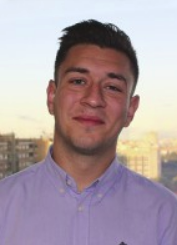
\includegraphics[width=1\textwidth]{juancar}
\end{minipage}      
\begin{minipage}{0.7\linewidth}
   \MyName{Juan Carlos Martín Sánchez} % Your Name here !
   \title{CV}
   \sepspace
   \noindent
   % Your email here
   \hfill  +34 619045231

   % Optionally your phone...
     \hfill juancarmartin1994@gmail.com  
 
   
   \hfill Disponibilidad en movilidad geográfica y coche propio.
   

\end{minipage}

%%%%%%%%%%%%%%%%%%%%%%%%%%%%%%%%%%%%%%%%%%%%%%%%%%%%%%%%%%%%%%%%%%%%%%%%%%%%%%%%
\NewPart{Experiencia Profesional}{}
\noindent


\textbf{{1. Babel Sistemas de la Información }{Feb 2018 - Sep 2018}\hspace{10pt}{Sysadmin/Devops}}

\tab Proyecto EtherOS del cliente BBVA en el que se pretende realizar una nube privada con distintos servicios de almacenamiento de ficheros, métricas, logs, alarmas... para los desarrolladores del BBVA. Formo parte del equipo de operaciones/devops de este proyecto, realizando tareas de automatización de procesos y despliegues de los servicios tanto en los entornos de preproducción como en los de producción. También me encargo del mantenimiento de la infraestructura del proyecto como nivel 2 a través del alarmado del propio servicio.
\sepspace

\textbf{{2. TechOnRails }{Sep 2018 - Actualidad}\hspace{10pt}{DevOps/Solution Architect}}

\tab Proyecto Sitra+ para Adif, este proyecto tiene como objevito el enrutamiento de los trenes a su llegada a las a principales estaciones españolas. Formo parte del equipo de Arquitectura, la cual es una UTE con Indra para proponer una solución en la nube para este enrutador. Mis tareas son: diseño de la arquitectura del enrutador, despliegue de aplicaciones, BBDD, mensajería, memorias caché, herramientas de tratamiento de logs en la nube, concretamente con la herramienta de Openshift, además de esta parte técnica tengo reuniones con el cliente para asesorarle en su infraestuctura y ayudarle en su transformación a este tipo de soluciones cloud.




%%%%%%%%%%%%%%%%%%%%%%%%%%%%%%%%%%%%%%%%%%%%%%%%%%%%%%%%%%%%%%%%%%%%%%%%%%%%%%%%
\NewPart{Education}{}
\noindent

\EducationEntry{Grado en Ingeniería de Computadores}{Sep 2013- Sep 2018}{Universidad Complutense de Madrid}{}
{IMG/complu}

\sepspace

\EducationEntry {Programa Erasmus}{Sep 2016 - Jul 2017}{Adam Mickiewicz University}{}{IMG/adam}

\sepspace

%%%%%%%%%%%%%%%%%%%%%%%%%%%%%%%%%%%%%%%%%%%%%%%%%%%%%%%%%%%%%%%%%%%%%%%%%%%%%%%%
\NewPart{Habilidades \& Lenguajes de programación}{}
\hspace{3mm}
\begin{minipage}[t]{0.33\textwidth} 

\begin{tabular}[t]{ l l }
\flag{IMG/flag/es}  & Nativo \\
\flag{IMG/flag/gb}  & Professional Proficiency \\
\end{tabular}

\sepspace

\end{minipage}
%
\begin{minipage}[t]{0.66\textwidth} 


\begin{tabular}[t]{l l}

Lenguajes de Scripting: Bash/Shell/Python \\
SDKs: Eclipse/xCode/Visual Studio \\
Herramientas: OPenshift/Docker/OpenStack/Jenkins \\
Sistemas Operativos: Ubuntu/Debian/RedHat/MacOS/Windows \\
Control de versiones: Git/Github/bitBucket \\
BBDD: Cassandra/MySql/PostgreSQL \\
Lenguajes de Programación: C/C++/Java/Python/Ansible/Swift \\
\end{tabular}



\end{minipage}





%%% References
%%% ------------------------------------------------------------

\end{document}
